\documentclass[a4paper, 12pt]{article}
\usepackage{cmap}
\usepackage{amssymb}
\usepackage{amsmath}
\usepackage{graphicx}
\usepackage{amsthm}
\usepackage{upgreek}
\usepackage{setspace}
\usepackage{color}
\usepackage[T2A]{fontenc}
\usepackage[utf8]{inputenc}
\usepackage[normalem]{ulem}
\usepackage{mathtext} % русские буквы в формулах
\usepackage[left=2cm,right=2cm, top=2cm,bottom=2cm,bindingoffset=0cm]{geometry}
\usepackage[english,russian]{babel}
\usepackage[unicode]{hyperref}
\newenvironment{Proof} % имя окружения
{\par\noindent{$\blacklozenge$}} % команды для \begin
{\hfill$\scriptstyle\boxtimes$}
\newcommand{\Rm}{\mathbb{R}}
\newcommand{\Cm}{\mathbb{C}}
\newcommand{\Z}{\mathbb{Z}}
\newcommand{\I}{\mathbb{I}}
\newcommand{\N}{\mathbb{N}}
\newcommand{\rank}{\operatorname{rank}}
\newcommand{\Ra}{\Rightarrow}
\newcommand{\ra}{\rightarrow}
\newcommand{\FI}{\Phi}
\newcommand{\Sp}{\text{Sp}}
\renewcommand{\leq}{\leqslant}
\renewcommand{\geq}{\geqslant}
\renewcommand{\alpha}{\upalpha}
\renewcommand{\beta}{\upbeta}
\renewcommand{\gamma}{\upgamma}
\renewcommand{\delta}{\updelta}
\renewcommand{\varphi}{\upvarphi}
\renewcommand{\phi}{\upvarphi}
\renewcommand{\tau}{\uptau}
\renewcommand{\lambda}{\uplambda}
\renewcommand{\psi}{\uppsi}
\renewcommand{\mu}{\upmu}
\renewcommand{\omega}{\upomega}
\renewcommand{\d}{\partial}
\renewcommand{\xi}{\upxi}
\renewcommand{\epsilon}{\upvarepsilon}
\newcommand{\intx}{\int\limits_{x_0}^x}
\newcommand\Norm[1]{\left\| #1 \right\|}
\newcommand{\sumk}{\sum\limits_{k=0}^\infty}
\newcommand{\sumi}{\sum\limits_{i=0}^\infty}
\newtheorem*{theorem}{Теорема}
\newtheorem*{cor}{Следствие}
\newtheorem*{lem}{Лемма}
\begin{document}
	\section*{Метод Лобачевского для наибольшего по модулю корня многочлена}
	\subsubsection*{Условие}
	Вычислить с точностью $\epsilon=10^{-1}$ наибольшую по модулю корень алгебраического уравнения $$2x^3-12x^2+6x +20 = 0.$$
	\subsubsection*{Алгоритм решения}
	Для решения задачи методом Лобачевского нам понадобятся следующие формулы:
	\begin{enumerate}
		\item соотношения для коэффициентов: 
		\begin{eqnarray}
		\begin{cases}
				a_0^{(1)} = a_0^2,\\
				a_1^{(1)} =2a_0a_2 - a_1^2,\\
				a_2^{(1)} = 2a_0a_4 - 2a_1a_3 + a_2^2,\\
				\dotfill\\
				a_n^{(1)} = (-1)^na_n^2
		\end{cases}
		\end{eqnarray}
		(конкретно эта формула позволяет перейти от итерации 0 к итерации 1, но для перехода от $k$ к $k+1$ соотношения такие же).\\\\
		Для нашего случая соотношения будут иметь вид
		\begin{eqnarray}
			\begin{cases}
			a_0^{(1)} = a_0^2,\\
			a_1^{(1)} =2a_0a_2 - a_1^2,\\
			a_2^{(1)} = - 2a_1a_3 + a_2^2,\\
			a_3^{(1)} = -a_3^2
		\end{cases}
		\end{eqnarray}
		\item формула для вычисления корней \begin{eqnarray}
			x_i\approx\sqrt[2^k]{ - \dfrac{a_i^{(k)}}{a_{i-1}^{(k)}}},\quad i =\overline{1,n}.
		\end{eqnarray}
	\end{enumerate} 
	\textbf{Замечание.} Метод Лобачевского после прохождения всего цикла возвращает значения корней \textit{по модулю}. Поэтому необходимо подстановкой в исходное уравнение проверить, с каким знаком нужно раскрывать модуль.\\\\
	Будем обозначать абсолютное значение наибольшего по модулю корня $x$ как $x_1 = |x|$.
	Для упрощения вычислений преобразуем данный в условии многочлен к приведенному виду (разделим на 2):
	$$x^3-6x^2+3x +10 = 0.$$
	Для решения методом Лобачевского удобно составить следующую таблицу (каждый столбец -- это коэффициенты, а в конце значение корня на каждой итерации):
	$$
		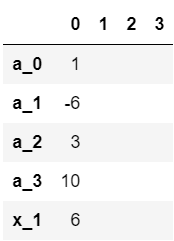
\includegraphics[scale=0.6]{img01}
	$$
	Мы переписали коэффициенты исходного многочлена и в последней строке посчитали корень $x_1$ по формуле (3) $$x_1 = - \dfrac{a_1}{a_0}.$$
	Далее воспользуемся соотношением для коэффициентов (2) и получим новые коэффициенты:
	$$\begin{cases}
		a_0^{(1)} = a_0^2 = 1,\\
		a_1^{(1)} =2a_0a_2 - a_1^2 = -30,\\
		a_2^{(1)} = - 2a_1a_3 + a_2^2 = 129,\\
		a_3^{(1)} = -a_3^2 = -100
	\end{cases}$$
	Посчитаем корень по формуле (3) $$x_1^{(1)} = \sqrt{- \dfrac{a_1^{(1)}}{a_0^{(1)}}} \approx 5.4772$$
	Заносим в таблицу:
	$$
		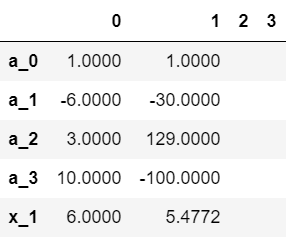
\includegraphics[scale=0.56]{img02}
	$$
	Вычислим погрешность: $$|x_1^{(1)} - x_1^{(0)}| = 0.228 > 10^{-1} = \epsilon.$$
	Так выглядит одна итерация. И пока модуль разности корней не будет меньше $\epsilon$, мы продолжаем итерации.\\\\
	Далее все действия повторяем. Коэффициенты снова считаем по соотношению (2), а корень теперь вычисляем по формуле (3) как $$x_1^{(2)} = \sqrt{\sqrt{- \dfrac{a_1^{(2)}}{a_0^{(2)}}}}\approx 5.0337$$
	$$
		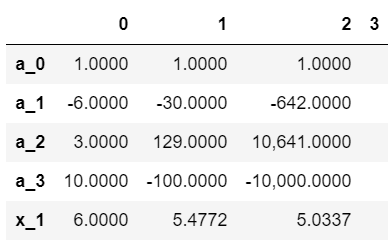
\includegraphics[scale=0.6]{img03}
	$$
	$$|x_1^{(2)} - x_1^{(1)}| = 0.4435 > 10^{-1} = \epsilon.$$
	Сделаем еще одну итерацию. Снова коэффициенты вычисляем по соотношению (2), а корень теперь уже по формуле (3) равен $$x_1^{(3)} = \sqrt[8]{- \dfrac{a_1^{(3)}}{a_0^{(3)}}}\approx 5.0004$$
	$$
		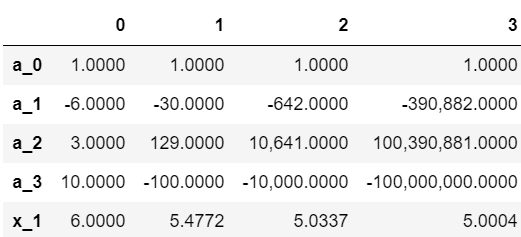
\includegraphics[scale=0.6]{img04}
	$$
	$$|x_1^{(3)} - x_1^{(2)}| = 0.0333 < 10^{-1} = \epsilon.$$
	В итоге мы нашли абсолютное значение наибольшего по модулю: $$|x| = x_1 \approx 5.0$$
	Необходимо проверить, какое из значений $x=5$ и $x=-5$ является корнем исходного уравнения. Подставим $x=5$:
	$$125 - 6\cdot 25 + 3\cdot 5 + 10 = 0.$$
	Можно также проверить и убедиться, что значение $x=-5$ не подходит. Следовательно, $x=5$ --- наибольший по модулю корень исходного уравнения.
\end{document}